\section{Question 2}
\subsection{Find the modal tooth length across the entire data set.}
\begin{lstlisting}
# clear the console area
cat("\014")

# clear the environment var area
rm(list = ls())

# Load the Tooth Growth data set
data(ToothGrowth

# Find the modal tooth length
modal_tooth_length1 = as.numeric(names(sort(
    table(ToothGrowth$len), decreasing = TRUE)[1]))
\end{lstlisting}
% 
\subsection{Mean tooth length for guinea pigs who were given their vitamins via orange juice}
% 
\begin{lstlisting}
# Calculate the mean tooth length for guinea pigs 
# given vitamins via orange juice
mean_tooth_length_orange = mean(
    ToothGrowth$len[ToothGrowth$supp == "OJ"])
mean_tooth_length_orange    
\end{lstlisting}
% 
\subsection{Create a side-by-side box-and-whisker plot:}
% 
\begin{lstlisting}
# Create a side-by-side box-and-whisker plot
# for tooth length by supplement type
boxplot(len ~ supp, data = ToothGrowth, 
        col = c("lightblue", "lightgreen"),
        xlab = "Supplement Type", ylab = "Tooth Length",
        main = "Tooth Length by Supplement Type")
legend("topright", 
        legend = c("Ascorbic Acid", "Orange Juice"), 
        fill = c("lightblue", "lightgreen"))
\end{lstlisting}
% 
% 
\begin{figure}[H]
    \centering
    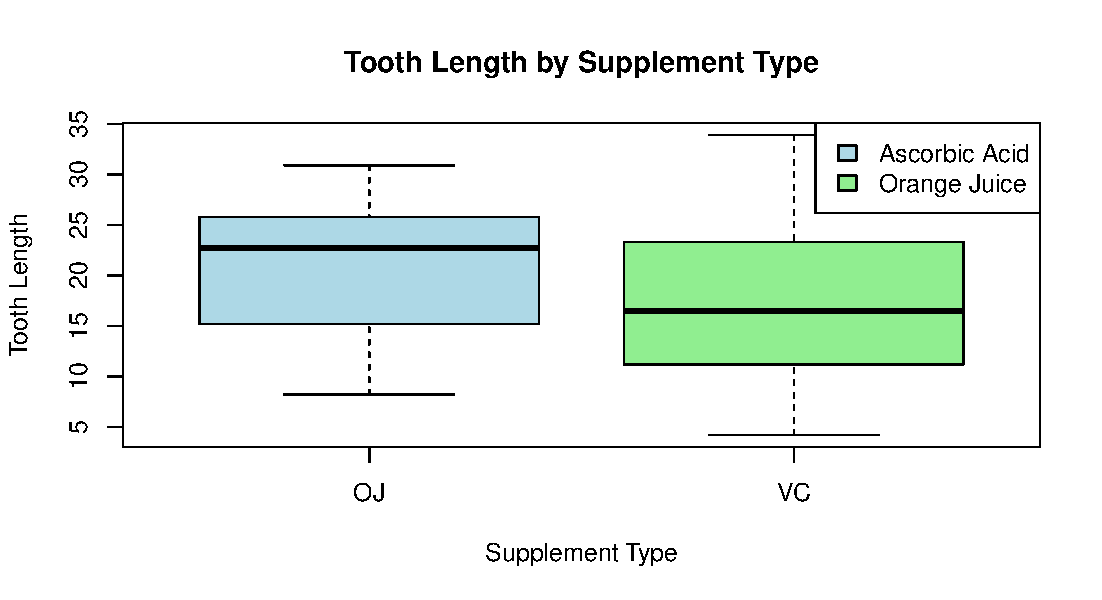
\includegraphics[width=0.8\textwidth]{img/ToothLength.pdf}
    % \caption{}
    % \label{fig:your-label}
\end{figure}
% 
% 
\subsection{Comment on which vitamin delivery approach is more effective:}
\paragraph{To determine which vitamin delivery approach is more effective in promoting tooth growth, you should analyze the box-and-whisker plot created in the previous step. Look at the distribution of tooth lengths for guinea pigs given vitamins via ascorbic acid and orange juice.
If the median tooth length for one group is higher than the other, it suggests that the corresponding supplement may be more effective.
Additionally, look for differences in the spread (interquartile range) and the presence of outliers. A supplement with a larger median, smaller spread, and fewer outliers may be considered more effective.}